\section{Quality Control}
\label{sec:QC}

%The section on quality control (QC) and quality assurance (QA) is grossly inadequate and needs major revision to be of any utility to a nonexpert user.  The monthly QC checks need to be described as well as the acceptance criteria for the QC check results and the procedures for documenting the QC check results.  Most of the section on QC checks appears to have been copied without attribution from a Bruker sales literature for the TENSOR II FTIR spectrometer.  It provides little useful information about the automated performance qualification (PQ) and operational qualification (OQ) routines for instrument validation.  This section needs to describe the specific tests involved in the PQ and OQ routines as well as the frequency of these tests, the acceptance criteria for the PQ and OQ test results, what to do if the criteria are not attained, and the procedure for documenting these test results in instrument logs.

Monthly quality control checks are performed to monitor the comparability, precision and stability of the TENSOR II FT-IR instrument over time. The TENSOR II spectrometer is prepared with automated performance qualification (PQ) test routines for instrument validation\cite{Bruker1}. 

\textbf{All details on PQ tests in this section are sourced from the OPUS software manual accessible via the Help menu of the OPUS software application}.

The PQ test for the spectrometer can not be deactivated, and the maximum validity period of a PQ test is 30 days. When the PQ test validity period expires, the instrument status in the OPUS software turns yellow and indicates a warning that the reliability of the measurement results is not ensured.

The PQ test protocol includes the following tests. This document details each test in Section \ref{subsec:individualPQ} below.

\begin{itemize}
    \item Signal-to-noise test: This test verifies that the signal-to-noise ratio is better than a specified limit.
    \item Deviation from 100\% line: This test verifies that the 100\% line does not shift on the long term.
    \item Interferogram peak amplitude: This test verifies that the interferogram peak amplitude is not below a certain limit.
    \item Energy distribution test: This test verifies, by means of different methods, the total energy of the spectrometer and its different components.
    \item Ice band test: This test verifies the leak tightness of liquid nitrogen-cooled detectors.
    %\item Sealing test: This test checks the water vapor signals during measuring time, and the absolute water vapor content in the optical path (only available with CONFOCHECK).
    \item Wavenumber accuracy test / X-axis frequency calibration test: This test verifies that the frequency calibration of the instrument is correct.
    \item Photometric accuracy test / Y-axis reproducibility test: This test verifies that the photometric accuracy is within specified limits. The test is performed by using one or two filter(s) with different absorbing properties.
    \begin{itemize}
        \item Glass Filter A Test
        \item Glass Filter B Test (not available for the spectrometer referenced in this QAPP)
    \end{itemize}
    %\item Position test: This test checks whether the HTS-XT x/y stage precisely approaches each measurement position of the microtiter plate (only available wtih the HTS-XT module).
\end{itemize}

Upon delivery of the TENSOR II FT-IR spectrometer, Bruker set up the test channels necessary for the spectrometer and delivered accessories. If additional accessories are purchased in the future, new test channels will need to be set up. For instructions on setting new test channels or PQ tests in the OPUS software, see the TENSOR II User Manual\cite{Bruker1} Section 5.11.4. %For instructions on running a PQ test, see TENSOR II User Manual\cite{Bruker1} Section 5.11.2.

\subsection{PQ Test Results}
The PQ Test Protocol contains the PQ test results. The first page summarizes the individual test results and the overall PASSED or FAILED test result is shown (see Figs. \ref{fig:samplePQ}-\ref{fig:samplePQ2}). Its remaining pages list the acquired spectra and the used measurement parameter values for each individual test of the PQ test.

The PQ test protocol PDF file is saved automatically in the following directory: \emph{Libraries \textbackslash Documents \textbackslash Public Documents \textbackslash Bruker \textbackslash OPUS\_[current version] \textbackslash Validation \textbackslash Reports}. This report is automatically displayed immediately after the PQ test is finished.

\begin{figure}[htp]
    \centering
    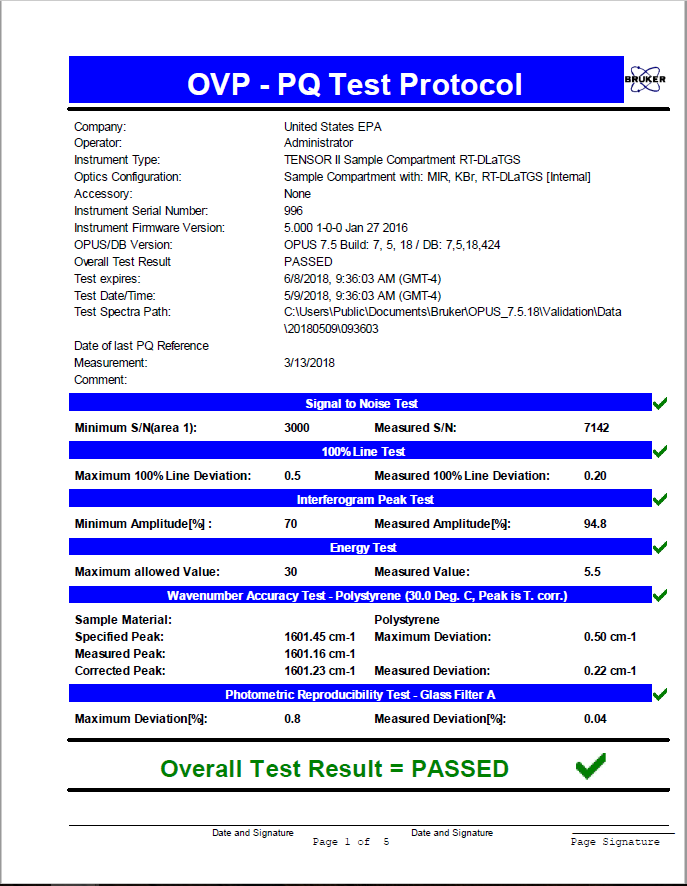
\includegraphics[width=6.5in]{PQtest.PNG}
    \caption{First page of a PQ Test Protocol file for the room-temperature detector.}
    \label{fig:samplePQ}
\end{figure}

\begin{figure}[htp]
    \centering
    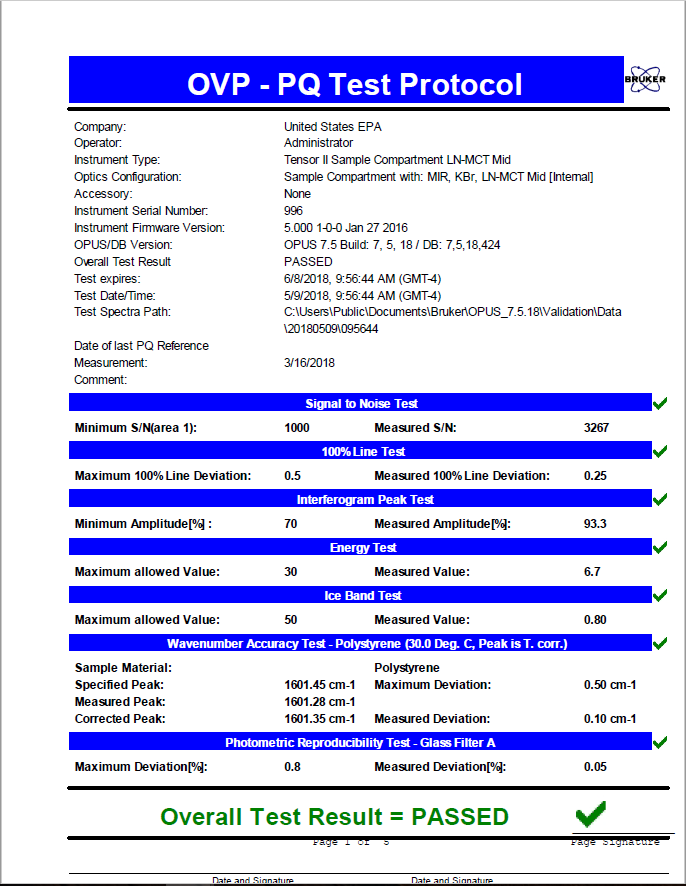
\includegraphics[width=6.5in]{PQtestMCT.PNG}
    \caption{First page of a PQ Test Protocol file for the liquid nitrogen-cooled detector.}
    \label{fig:samplePQ2}
\end{figure}

\subsection{Individual tests in the PQ test protocol}
\label{subsec:individualPQ}
\subsubsection{Signal to Noise Test}
The signal-to-noise ratio test determines the sensitivity of the spectrometer by calculating the average signal-to-noise ratio of ten 100\% spectra.

The S/N ratio is determined by collecting and analyzing a 100\% spectrum. A 100\% spectrum is the ratio of two successively acquired single-channel spectra with no sample in the sample compartment. The ratio of these two single-channel spectra is used to generate a transmission spectrum. The S/N ratio is calculated by the OPUS Signal-to-Noise Ratio command from the Evaluate menu, using peak-to-peak by means of the quadratic parabola fit option. In order to get a reliable result 10 spectra are measured (reference and sample). The S/N ratio is calculated separately for each spectrum, using the mean value of all 10 results. 

\subsubsection{Deviation from 100\% Line Test}
This test measures the maximum deviation of a 100\% line within a larger frequency range. The average determined by 10 measurements must not exceed the predefined limit of 0.5, defined by the instrument manufacturer.

\subsubsection{Interferogram Peak Test}
The interferogram peak amplitude test is a long-term stability test that compares the amplitude of a measured interferogram to that of the reference interferogram stored by the manufacturer. The amplitude of the reference interferogram corresponds to 100\%. In the PQ test the same measurement is repeated and the interferogram amplitude of this test spectrum is compared to the interferogram amplitude of the reference interferogram. The amplitude of the test interferogram is indicated in the PQ test report relative to the reference value and must not fall below 70\% of the reference interferogram. 

\subsubsection{Energy Distribution Test}
\label{subsubsec:energytest}
The energy distribution test is a long-term stability test that compares the amplitude of a measured single-channel spectrum to that of a reference single-channel spectrum stored at installation. The integral over the total reference single-channel spectrum is set to 100\%. If the power of the spectrometer source decreases, e.g., the distance between the two single-channel spectra will increase. Therefore, this test can be used to detect changes in the source power.

The decrease in the integral of the single-channel spectrum must not exceed 30\% of the stored reference spectrum.

The reference spectra can be re-measured after instrument re-alignment or optical source changes.

\subsubsection{Ice Band Test}
If the vacuum of a liquid nitrogen-cooled detector decreases, the ice band caused by condensed water vapor is observable in the single-channel spectrum. The ice band test compares the integral in the ice band region (3485--3050 $cm^{-1}$) with the integral of the reference spectrum measured for the PQ test. The integral should not exceed a 50\% difference from the manufacturer's reference. This test is part of the energy test.

\subsubsection{X-Axis Frequency Calibration Test (Wavenumber Accuracy Test)}
The x-axis frequency calibration test ensures that the frequency calibration of the instrument is within the specified limits.

If possible, water vapor is used to determine the wavenumber accuracy. Water vapor has an extremely narrow band, and allows the x-axis position to be measured to a very high degree of accuracy. The instrument uses a high-resolution setting to ensure that the water vapor band (at 1554.353 $cm^{-1}$ for mid-IR) is completed resolved. The maximum deviation of the measured peak is 0.50 $cm^{-1}$ from the specified band at 1554.353 $cm^{-1}$.

It is also possible to measure the spectrum of the mounted filter, instead of water vapor, if the water vapor concentration is too low. In this case, a polystyrene standard sample can be used, with a specified peak at 1601.45 $cm^{-1}$. The standard is on the internal validation unit.

\subsubsection{Y-Axis Reproducibility Test (Photometric Accuracy)}
The y-axis reproducibility test is a long-term stability test that compares the total intensity values of glass filter spectra to those of the reference spectra stored at installation.

A glass filter transmission spectrum is used to test the precision of the y-axis. The test spectra of glass filters are compared to the stored reference spectra by calculating the mean difference over a large spectral range (4000--2000 $cm^{-1}$ for mid-IR). The maximum deviation of the mean difference is 0.8\%.

%To monitor instrument stability, the empty chamber background signal is collected at the start of each week of experiments. This signal is matched with first background signal taken from the instrument's setup. The signals should overlap exactly or be closely parallel.